\section{Introduction}

Single Instruction, Multiple Data (SIMD) architectures are designed to apply the same instruction to multiple data points simultaneously. 
In contrast, languages like C and C++ are primarily oriented toward single-threaded execution, supporting parallelism through well-known solutions such as OpenMP and \texttt{std::thread}. 
However, leveraging SIMD hardware poses unique challenges, as it typically requires either manual low-level programming or reliance on compilers to automatically vectorize code.

ISPC (Intel SPMD Program Compiler) is a C-based programming language specifically tailored for parallel computation. 
It employs a Single Program, Multiple Data (SPMD) model to facilitate parallelism across SIMD lanes, while also providing tasks to enable parallelism across multiple cores.

The ISPC compiler, built on the LLVM framework, is freely available and well-documented, making it accessible for developers looking to optimize their applications.
\begin{figure}[H]
    \centering
    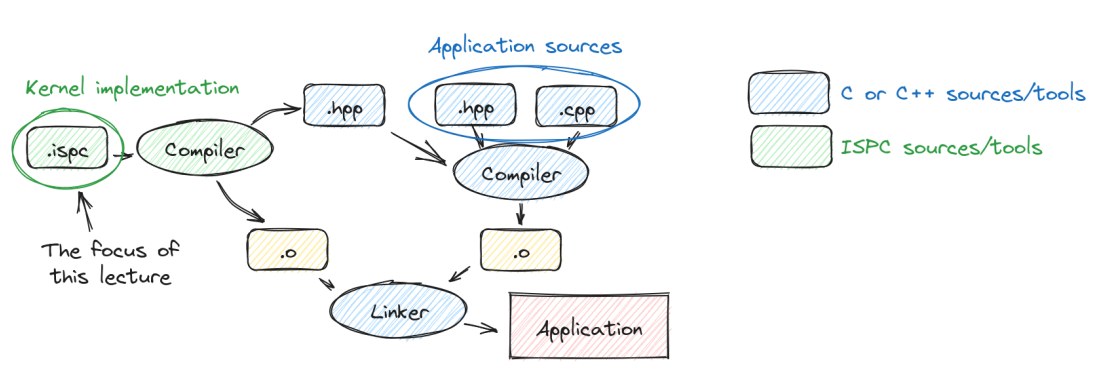
\includegraphics[width=0.75\linewidth]{images/ispc.png}
    \caption{ISPC compiler}
\end{figure}
The ISPC computation model allows application code to be executed by a single processor as usual, while functions implemented in ISPC are executed by a gang of program instances, enabling efficient use of SIMD capabilities.